\documentclass[11pt]{article}
\setlength{\oddsidemargin}{0in}
\setlength{\evensidemargin}{0in}
\setlength{\textwidth}{6.5in}

\usepackage{float}
\usepackage{fancyhdr}
\pagestyle{fancy}
\usepackage{amsmath,amsfonts,amssymb}
\usepackage{epsfig}
\usepackage{subfigure}
\usepackage{placeins}
\usepackage{amsmath}
\usepackage[usenames,dvipsnames,svgnames,table]{xcolor}
\usepackage{amssymb}
\usepackage{setspace}
\usepackage{graphicx} % Include figure files
\usepackage{times}
\usepackage{amsthm}
\usepackage{hyperref}
\usepackage{enumitem}
\hypersetup{bookmarks=true, unicode=false, pdftoolbar=true, pdfmenubar=true, pdffitwindow=false, pdfstartview={FitH}, pdfcreator={Daniel Larremore}, pdfproducer={Daniel Larremore}, pdfkeywords={} {} {}, pdfnewwindow=true, colorlinks=true, linkcolor=blue, citecolor=Green, filecolor=magenta, urlcolor=cyan,}
\usepackage[parfill]{parskip}
\usepackage{tcolorbox}
\tcbuselibrary{breakable}

\graphicspath{{../Notes/PythonFigs/}{./}}

\newcommand{\e}{\mathrm{e}}
\renewcommand{\d}{\mathrm{d}}
\newcommand{\erf}{\mathop\mathrm{erf}}
\newcommand{\erfc}{\mathop\mathrm{erfc}}
\newcommand{\xmin}{\ensuremath{x_{\min}}}
\newcommand{\ntail}{\ensuremath{n_{\rm tail}}}

\newcommand{\Q}[1]{\footnote{\textcolor{blue}{#1}}}

\begin{document}

\lhead{{\bf Mathematical \& Computational Modeling of Infectious Diseases \\ 
Homework 2}}
\rhead{{\bf D.B.\ Larremore\\2024}}
\renewcommand{\headrulewidth}{0.4pt}

{\bf Instructions:} 
\begin{itemize}[itemsep=-7pt]
	\item Please turn in a single PDF file. 
	\item Please share a link to your code, but do not attach the actual code. 
	\item Handwritten math (scanned and included in a PDF) is fine, but please watch out for 10MB+ file sizes!
\end{itemize}
\vspace{0.1in}\hrule

\begin{enumerate}
	\item The goal of this problem is to develop flexibility with your Forward Euler code, and to learn a bit about the effect of step size on the accuracy of the solution.
	
\begin{enumerate}[label=\alph*.]
	\item Using your Forward Euler method, simulate the solution to the {\it normalized} SIS model discussed in class (Week 3) using $\beta=3$ and $\gamma=2$, and with $(s_0, i_0) = (0.99, 0.01)$. Create three plots ranging from $t=0$ to $t=25$. On the first, simulate using a step size $\Delta t=2$. On the second, use $\Delta t =1$. On the third, use $\Delta t = \tfrac{1}{2}$. In each plot, show only your solution's $I(t)$ in a red solid line, labeled as ``Forward Euler'', and then also plot the analytical solution from class in a black dashed line, labeled as ``Analytical.'' Please also set the y-axis range to $[0,0.5]$. 
	
	\begin{tcolorbox}
		\textbf{Solution}: For clarity, since we are using the normalized SIS model and a total population $N$ was not specified in the problem, instead of plotting $I(t)$, we will be plotting $i(t)$ as an infected fraction.
	\end{tcolorbox}

	\begin{figure}[H]
		\centering
		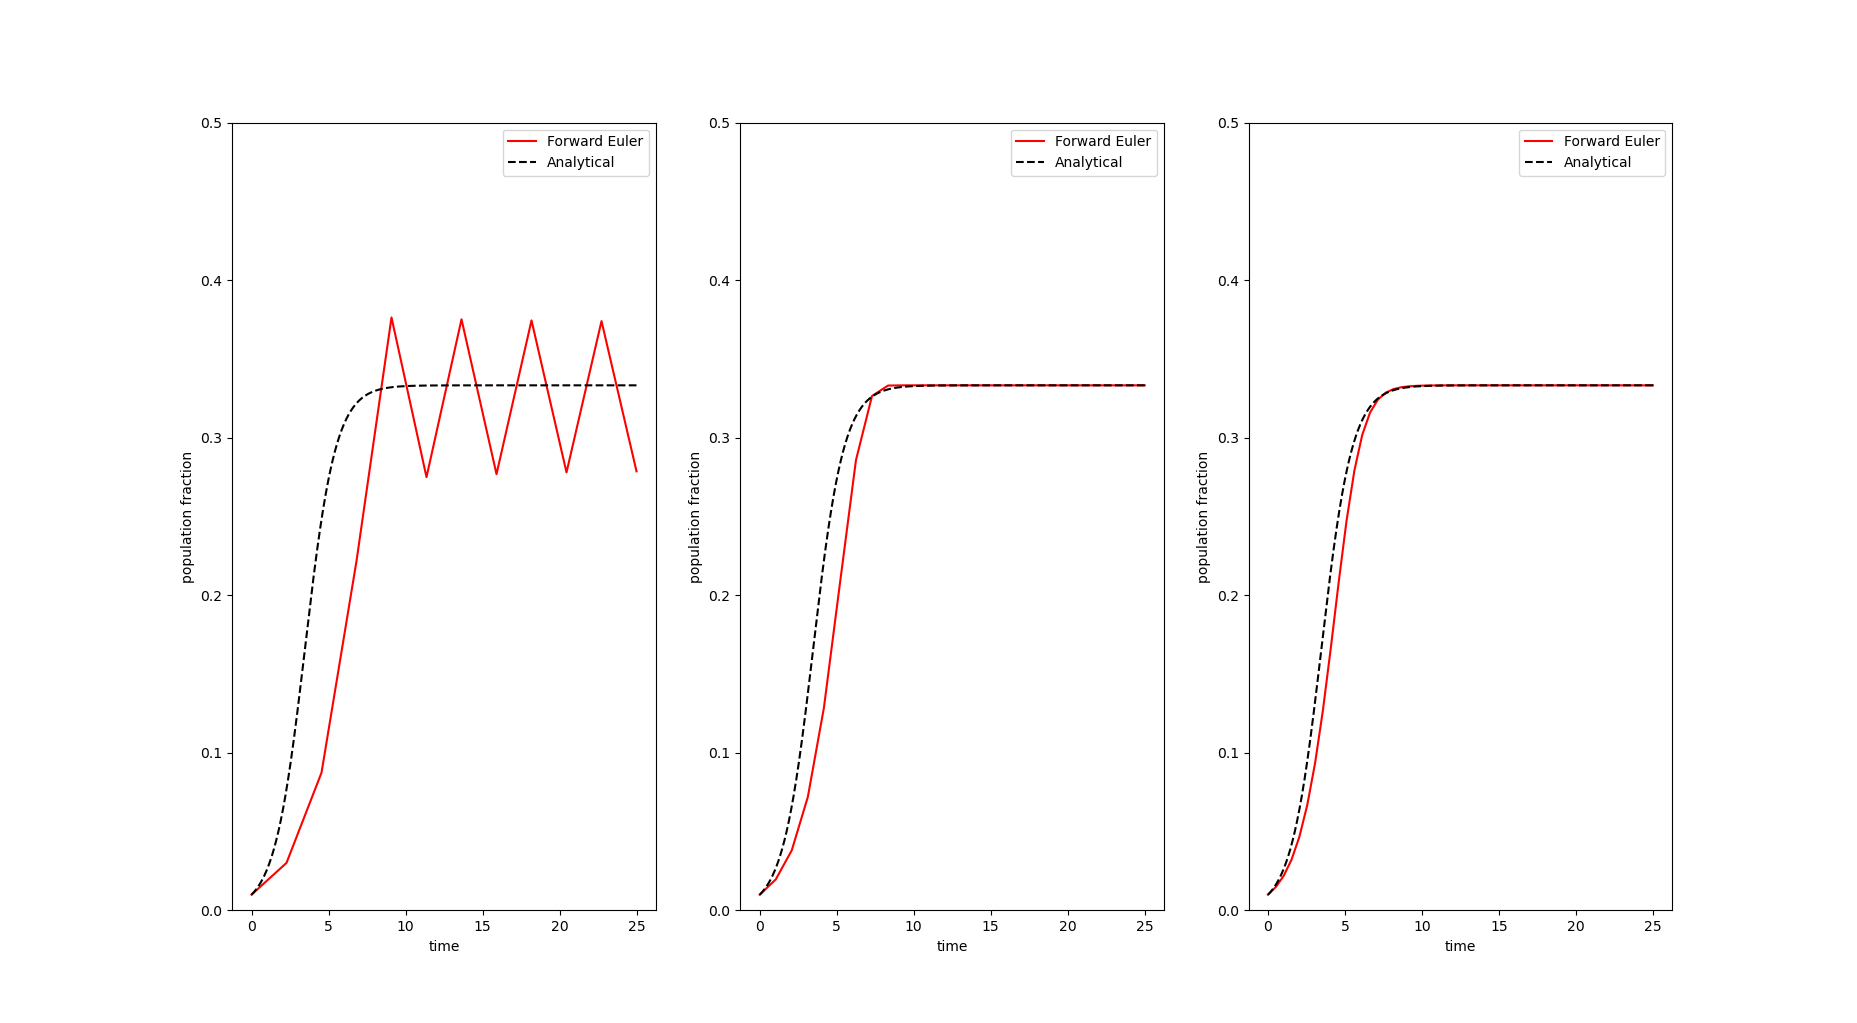
\includegraphics[scale=0.35]{hw2p1.png}
		\caption{SIS model with parameters $(\beta, \gamma)=(3, 2)$ and initial condition $i_0=0.01$ simulated using Forward Euler with different resolutions. From left to right, the time steps are $\Delta t = (2, 1, \frac{1}{2})$}.
	\end{figure}
	
	\item Comment on what you see in your three plots. How does the step size affect our solution?
	\begin{tcolorbox}
		\textbf{Solution}: For $\Delta t = 2$, the timestep is so large that it periodically overshoots and undershoots the equilibrium position, causing jagged oscillations, which is problematic for solutions. For $\Delta t =1$ the solution reaches equilibrium, but the transition region is a poor match. For $\Delta t=1/2$, the solution is quite close, but has the most issue in the transition region. Note that for the stability that we want, we require $\Delta t < \lambda = \beta-\gamma$, so we may either shrink the timestep or, based on the parameters used, we can boost the timestep up to that limit if we wanted speed and efficiency.
	\end{tcolorbox}
	\item Define the maximum absolute error for a simulation using a particular $\Delta t$ as $$E(\Delta t) = \max_{t} \big | I_{\text{Euler}, \Delta t} (t) - I_\text{analytical}(t) \big |\ .$$ Write a function that runs the appropriate simulation, computes the analytical solution, and returns $E$ without plotting. Share a link to your code for this problem.
	\begin{tcolorbox}
		\textbf{Solution}: Code provided at \href{https://github.com/WilliamMagrogan/InfectiousDiseaseModeling}{here} under the HW2 directory, or copy/paste the link into the web browser of your choice: https://github.com/WilliamMagrogan/InfectiousDiseaseModeling and navigate to HW2.
	\end{tcolorbox}
	\item Create a plot on log-log axes showing $E(\Delta t)$ vs $\Delta t$ for values $$\Delta t \in \{2,1,\tfrac{1}{2},\tfrac{1}{4},\tfrac{1}{8},\tfrac{1}{16},\tfrac{1}{32}\}$$
	\begin{tcolorbox}
		\textbf{Solution}: The graph is provided below in Fig. \ref{fig:dtscaling}. The slope is very nearly $1$ in logspace, indicating that the absolute error over the solution for this problem using Forward Euler is $O((\Delta t)^1)$, mean as $\Delta t$ gets small, the error scales linearly with $\Delta t$.
	\end{tcolorbox}
	\begin{figure}[H]
		\centering
		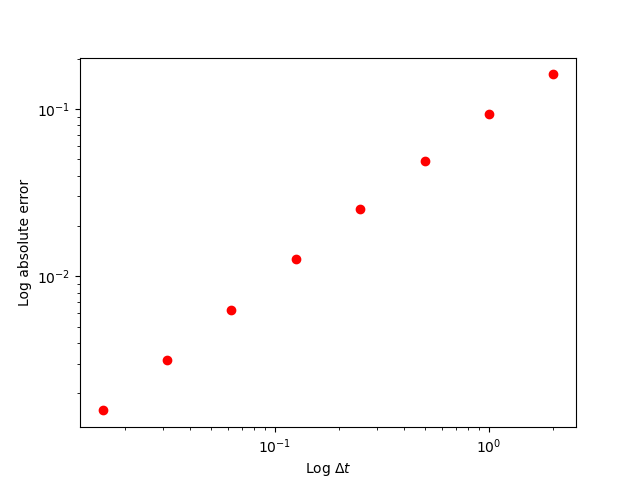
\includegraphics[scale=0.8]{hw2p1c.png}
		\caption{Plot detailing trend of absolute error with decreasing $\Delta t$.}
		\label{fig:dtscaling}
	\end{figure}
	\item Comment on what you observe in this plot, and comment on cases when you would want a larger or smaller step size, and why? Imagining yourself in an advisory position in your community, can you think of any scenario where there is a connection between the step size of your simulation and the ethics of your advice?
	\begin{tcolorbox}
		\textbf{Solution}: The main thing to notice is that sufficiently small $\Delta t$, the error scales linearly. This continues until machine precision is reached, though that is rarely reached. It turns out that to maintain stability, a stepsize needs to be smaller than the reciprocal of the largest gradient that needs to be resolved, and small enough to keep the overall error sufficiently small for the purposes. Though, depending on the model, you want to keep the timestep large enough to make a viably fast simulation. So, in sum, keep the step small enough to maintain stability and error requirements, but only barely smaller than that. 
		
		We note that ethical concerns arise if stability is breached and you get non-existent oscillations or artifacts, as that will influence policy behavior and potential interventions, and poor accuracy may lead to mis-allocations of resources when taking plans of action.
	\end{tcolorbox}
	
\end{enumerate}

\clearpage
\item The goal of this problem is to confront the differences between the leaky model of vaccination and the all-or-nothing model of vaccination. A secondary goal is to give you a chance to get creative in how you draw connections between relevant real-world questions and the models we discuss in class. 

``Good news, everyone!'' remarks the chair of your vaccine rollout committee. It is early 2031, and you are on a team considering policy choices around vaccination for your community in the middle of a pandemic. ``Our vaccines are in and they have $VE=0.8$,'' she continues. Everyone claps because that number seems pretty high. ``As you know, we've got a tough road ahead. We have enough vaccines for only 50\% of our population, we don't know whether we should think of this as a Leaky or All-or-Nothing vaccine, and we're not sure if the latest variant will have $R_0=3$, $R_0=4$, or $R_0=5$. Still, it looks like the typical infection is lasting 14 days, which is the same for all variants.''
\begin{enumerate}[label=\alph*.]
	\item Assuming SIR dynamics and no prior infections in your community, do you have any hope of reaching herd immunity through vaccination, given what you know? Why or why not?
	\begin{tcolorbox}
		\textbf{Solution}: Considering that there have been no prior infections in the community, we should assume that, at present, there are no people in the recovered category. Considering the normalized SIR model, if we want the concentration of infections to decrease, we require that
		\begin{equation*}
			\dot{\iota} = (\beta s-\gamma)\iota.
		\end{equation*}
		Since we consider a small, but nonzero density of infections to start, we have that $0<\iota_0 = \epsilon <<1$, then for the infection rate to decrease, $s_0<\frac{\gamma}{\beta}=\frac{1}{R_0}$. The fraction that needs to be vaccinated (recovered), then, that is needed for herd immunity is $1-\rho_{\text{vacc}}<\frac{1}{R_0}$ and so we need
		\begin{equation*}
			\rho_{\text{vacc}}>1-\frac{1}{R_0}.
		\end{equation*}
		The corresponding herd immunity thresholds (HITs) are $(66.\bar{6}\%, 75\%,$ and $80\%)$ for $R_0=(3, 4, 5)$ respectively. If there are only vaccines available to immunize at most $50\%$ of the population, then herd immunity via vaccination is not an option.
	\end{tcolorbox}
	\item Someone pipes up in the back of the meeting ``Hey how many people are going to become infected anyway, even with the vaccine, when this wave rolls through?'' You immediately sense that this is something you can answer, because you have taken Computational and Mathematical Modeling of Infectious Diseases, and recall that HW 2 Question 2 was something like this... Your daydreaming about class is interrupted: ``...and do we care if we're using the Leaky or All-or-Nothing model, or what the value of $R_0$ is?'' You reply... [please write 3 sentences of what you might say to your colleague in the meeting].
	\begin{tcolorbox}
		\textbf{Solution}: 
		"Good question, depending on the suite of models used to estimate, the number of people infected usually increases with, and is very sensitive to, $R_0$. The quality of of the vaccination will affect the estimate a bit differently as well. All-or-nothing models confer absolute immunity, and those vaccinated can never contribute to the total infections, and conversely, with a leaky model, all vaccinated are still liable to contribute to the load."
	\end{tcolorbox}
	\item After the meeting, your chair comes up to you, and in a way you cannot refuse, kindly says, ``I liked what you said about how we might think about the differences between the different vaccine models, and how they might interact with $R_0$ in our little community of $300,000$. Can I ask you to write up a quick one-page summary with a few graphs to show how much the model does or doesn't matter in our scenarios?''  OOOOF you think: it is the future and so you were hoping to go electric-snowboarding, but this one-pager is important. [Write the one-pager that helps {\it a mathematically savvy person from the general public} to understand your projections about infections in all three $R_0$ scenarios and using both vaccine models. Be sure to include an executive summary sentence at the top of the report so your chair and read it aloud at a press conference if someone asks!]\footnote{Here is a good opportunity to apply what you've learned in the previous problem: what step size is sufficient?}
	\begin{tcolorbox}
		\textbf{Solution}:
	\end{tcolorbox}
\end{enumerate}

\clearpage
\item (Grad / EC): The goal of this problem is to get you to think about additional flavors of models that build on the SIR model backbone, and practice writing down flow diagrams and systems of differential equations. For each of the following situations please (i) draw a flow diagram with the SIR backbone in black, (ii) include any modifications in a second color, and (iii) write out your differential equations using the same color scheme. 
\begin{enumerate}
	\item Suppose that we want to model the possibility that the natural history of infection means that a person is infected {\it but not infectious} before becoming infected-and-infectious. Let the typical {\it latent} period---the time between exposure and infectiousness---last for $q$ days. Use the letter $E$ for this new compartment. Draw a flow diagram for the non-normalized system, and write a set of corresponding differential equations. 
	\begin{tcolorbox}
		\textbf{Solution}:
	\end{tcolorbox}
	\item Suppose that we want to model Hospitalization, with the following assumption: Infected folks either recover directly {\it or} they are hospitalized first and then recover. Let the direct recovery rate be $\gamma$, and suppose that there are 4 direct recoveries for every 1 hospitalization. Let the typical duration of a hospitalization be $\delta$ days. Use the letter $h$ for the hospitalized compartment. Draw a flow diagram for the normalized system, and write a set of corresponding differential equations. You should assume that folks in the hospital do not come into contact with anyone else during their hospital stay.
	\begin{tcolorbox}
		\textbf{Solution}:
	\end{tcolorbox}
	\item Suppose that we want to model an infectious disease that afflicts a growing population of bacteria, such that the infection follows an SIR model, the bacteria grow according to a logistic growth model with intrinsic growth rate $\alpha$ and carrying capacity $K$. Let all bacteria reproduce, but suppose that susceptible and recovered bacteria produce susceptible progeny, while infected bacteria produce infected progeny. The carrying capacity is shared by all three bacteria. 
	\begin{tcolorbox}
		\textbf{Solution}:
	\end{tcolorbox}
\end{enumerate}

\end{enumerate}

\end{document}